% Options for packages loaded elsewhere
\PassOptionsToPackage{unicode}{hyperref}
\PassOptionsToPackage{hyphens}{url}
\PassOptionsToPackage{dvipsnames,svgnames,x11names}{xcolor}
%
\documentclass[
  letterpaper,
  DIV=11,
  numbers=noendperiod]{scrreprt}

\usepackage{amsmath,amssymb}
\usepackage{iftex}
\ifPDFTeX
  \usepackage[T1]{fontenc}
  \usepackage[utf8]{inputenc}
  \usepackage{textcomp} % provide euro and other symbols
\else % if luatex or xetex
  \usepackage{unicode-math}
  \defaultfontfeatures{Scale=MatchLowercase}
  \defaultfontfeatures[\rmfamily]{Ligatures=TeX,Scale=1}
\fi
\usepackage{lmodern}
\ifPDFTeX\else  
    % xetex/luatex font selection
\fi
% Use upquote if available, for straight quotes in verbatim environments
\IfFileExists{upquote.sty}{\usepackage{upquote}}{}
\IfFileExists{microtype.sty}{% use microtype if available
  \usepackage[]{microtype}
  \UseMicrotypeSet[protrusion]{basicmath} % disable protrusion for tt fonts
}{}
\makeatletter
\@ifundefined{KOMAClassName}{% if non-KOMA class
  \IfFileExists{parskip.sty}{%
    \usepackage{parskip}
  }{% else
    \setlength{\parindent}{0pt}
    \setlength{\parskip}{6pt plus 2pt minus 1pt}}
}{% if KOMA class
  \KOMAoptions{parskip=half}}
\makeatother
\usepackage{xcolor}
\setlength{\emergencystretch}{3em} % prevent overfull lines
\setcounter{secnumdepth}{2}
% Make \paragraph and \subparagraph free-standing
\ifx\paragraph\undefined\else
  \let\oldparagraph\paragraph
  \renewcommand{\paragraph}[1]{\oldparagraph{#1}\mbox{}}
\fi
\ifx\subparagraph\undefined\else
  \let\oldsubparagraph\subparagraph
  \renewcommand{\subparagraph}[1]{\oldsubparagraph{#1}\mbox{}}
\fi

\usepackage{color}
\usepackage{fancyvrb}
\newcommand{\VerbBar}{|}
\newcommand{\VERB}{\Verb[commandchars=\\\{\}]}
\DefineVerbatimEnvironment{Highlighting}{Verbatim}{commandchars=\\\{\}}
% Add ',fontsize=\small' for more characters per line
\usepackage{framed}
\definecolor{shadecolor}{RGB}{241,243,245}
\newenvironment{Shaded}{\begin{snugshade}}{\end{snugshade}}
\newcommand{\AlertTok}[1]{\textcolor[rgb]{0.68,0.00,0.00}{#1}}
\newcommand{\AnnotationTok}[1]{\textcolor[rgb]{0.37,0.37,0.37}{#1}}
\newcommand{\AttributeTok}[1]{\textcolor[rgb]{0.40,0.45,0.13}{#1}}
\newcommand{\BaseNTok}[1]{\textcolor[rgb]{0.68,0.00,0.00}{#1}}
\newcommand{\BuiltInTok}[1]{\textcolor[rgb]{0.00,0.23,0.31}{#1}}
\newcommand{\CharTok}[1]{\textcolor[rgb]{0.13,0.47,0.30}{#1}}
\newcommand{\CommentTok}[1]{\textcolor[rgb]{0.37,0.37,0.37}{#1}}
\newcommand{\CommentVarTok}[1]{\textcolor[rgb]{0.37,0.37,0.37}{\textit{#1}}}
\newcommand{\ConstantTok}[1]{\textcolor[rgb]{0.56,0.35,0.01}{#1}}
\newcommand{\ControlFlowTok}[1]{\textcolor[rgb]{0.00,0.23,0.31}{#1}}
\newcommand{\DataTypeTok}[1]{\textcolor[rgb]{0.68,0.00,0.00}{#1}}
\newcommand{\DecValTok}[1]{\textcolor[rgb]{0.68,0.00,0.00}{#1}}
\newcommand{\DocumentationTok}[1]{\textcolor[rgb]{0.37,0.37,0.37}{\textit{#1}}}
\newcommand{\ErrorTok}[1]{\textcolor[rgb]{0.68,0.00,0.00}{#1}}
\newcommand{\ExtensionTok}[1]{\textcolor[rgb]{0.00,0.23,0.31}{#1}}
\newcommand{\FloatTok}[1]{\textcolor[rgb]{0.68,0.00,0.00}{#1}}
\newcommand{\FunctionTok}[1]{\textcolor[rgb]{0.28,0.35,0.67}{#1}}
\newcommand{\ImportTok}[1]{\textcolor[rgb]{0.00,0.46,0.62}{#1}}
\newcommand{\InformationTok}[1]{\textcolor[rgb]{0.37,0.37,0.37}{#1}}
\newcommand{\KeywordTok}[1]{\textcolor[rgb]{0.00,0.23,0.31}{#1}}
\newcommand{\NormalTok}[1]{\textcolor[rgb]{0.00,0.23,0.31}{#1}}
\newcommand{\OperatorTok}[1]{\textcolor[rgb]{0.37,0.37,0.37}{#1}}
\newcommand{\OtherTok}[1]{\textcolor[rgb]{0.00,0.23,0.31}{#1}}
\newcommand{\PreprocessorTok}[1]{\textcolor[rgb]{0.68,0.00,0.00}{#1}}
\newcommand{\RegionMarkerTok}[1]{\textcolor[rgb]{0.00,0.23,0.31}{#1}}
\newcommand{\SpecialCharTok}[1]{\textcolor[rgb]{0.37,0.37,0.37}{#1}}
\newcommand{\SpecialStringTok}[1]{\textcolor[rgb]{0.13,0.47,0.30}{#1}}
\newcommand{\StringTok}[1]{\textcolor[rgb]{0.13,0.47,0.30}{#1}}
\newcommand{\VariableTok}[1]{\textcolor[rgb]{0.07,0.07,0.07}{#1}}
\newcommand{\VerbatimStringTok}[1]{\textcolor[rgb]{0.13,0.47,0.30}{#1}}
\newcommand{\WarningTok}[1]{\textcolor[rgb]{0.37,0.37,0.37}{\textit{#1}}}

\providecommand{\tightlist}{%
  \setlength{\itemsep}{0pt}\setlength{\parskip}{0pt}}\usepackage{longtable,booktabs,array}
\usepackage{calc} % for calculating minipage widths
% Correct order of tables after \paragraph or \subparagraph
\usepackage{etoolbox}
\makeatletter
\patchcmd\longtable{\par}{\if@noskipsec\mbox{}\fi\par}{}{}
\makeatother
% Allow footnotes in longtable head/foot
\IfFileExists{footnotehyper.sty}{\usepackage{footnotehyper}}{\usepackage{footnote}}
\makesavenoteenv{longtable}
\usepackage{graphicx}
\makeatletter
\def\maxwidth{\ifdim\Gin@nat@width>\linewidth\linewidth\else\Gin@nat@width\fi}
\def\maxheight{\ifdim\Gin@nat@height>\textheight\textheight\else\Gin@nat@height\fi}
\makeatother
% Scale images if necessary, so that they will not overflow the page
% margins by default, and it is still possible to overwrite the defaults
% using explicit options in \includegraphics[width, height, ...]{}
\setkeys{Gin}{width=\maxwidth,height=\maxheight,keepaspectratio}
% Set default figure placement to htbp
\makeatletter
\def\fps@figure{htbp}
\makeatother

% Soul package to handle highlighting (see hl.py3 filter)
\usepackage{soul}

% For tables generated by the gt package
\usepackage{colortbl}
\KOMAoption{captions}{tableheading}
\makeatletter
\@ifpackageloaded{tcolorbox}{}{\usepackage[skins,breakable]{tcolorbox}}
\@ifpackageloaded{fontawesome5}{}{\usepackage{fontawesome5}}
\definecolor{quarto-callout-color}{HTML}{909090}
\definecolor{quarto-callout-note-color}{HTML}{0758E5}
\definecolor{quarto-callout-important-color}{HTML}{CC1914}
\definecolor{quarto-callout-warning-color}{HTML}{EB9113}
\definecolor{quarto-callout-tip-color}{HTML}{00A047}
\definecolor{quarto-callout-caution-color}{HTML}{FC5300}
\definecolor{quarto-callout-color-frame}{HTML}{acacac}
\definecolor{quarto-callout-note-color-frame}{HTML}{4582ec}
\definecolor{quarto-callout-important-color-frame}{HTML}{d9534f}
\definecolor{quarto-callout-warning-color-frame}{HTML}{f0ad4e}
\definecolor{quarto-callout-tip-color-frame}{HTML}{02b875}
\definecolor{quarto-callout-caution-color-frame}{HTML}{fd7e14}
\makeatother
\makeatletter
\@ifpackageloaded{bookmark}{}{\usepackage{bookmark}}
\makeatother
\makeatletter
\@ifpackageloaded{caption}{}{\usepackage{caption}}
\AtBeginDocument{%
\ifdefined\contentsname
  \renewcommand*\contentsname{Índice}
\else
  \newcommand\contentsname{Índice}
\fi
\ifdefined\listfigurename
  \renewcommand*\listfigurename{Lista de Figuras}
\else
  \newcommand\listfigurename{Lista de Figuras}
\fi
\ifdefined\listtablename
  \renewcommand*\listtablename{Lista de Tabelas}
\else
  \newcommand\listtablename{Lista de Tabelas}
\fi
\ifdefined\figurename
  \renewcommand*\figurename{Figura}
\else
  \newcommand\figurename{Figura}
\fi
\ifdefined\tablename
  \renewcommand*\tablename{Tabela}
\else
  \newcommand\tablename{Tabela}
\fi
}
\@ifpackageloaded{float}{}{\usepackage{float}}
\floatstyle{ruled}
\@ifundefined{c@chapter}{\newfloat{codelisting}{h}{lop}}{\newfloat{codelisting}{h}{lop}[chapter]}
\floatname{codelisting}{Listagem}
\newcommand*\listoflistings{\listof{codelisting}{Lista de Listagens}}
\makeatother
\makeatletter
\makeatother
\makeatletter
\@ifpackageloaded{caption}{}{\usepackage{caption}}
\@ifpackageloaded{subcaption}{}{\usepackage{subcaption}}
\makeatother
\ifLuaTeX
\usepackage[bidi=basic]{babel}
\else
\usepackage[bidi=default]{babel}
\fi
\babelprovide[main,import]{portuguese}
% get rid of language-specific shorthands (see #6817):
\let\LanguageShortHands\languageshorthands
\def\languageshorthands#1{}
\ifLuaTeX
  \usepackage{selnolig}  % disable illegal ligatures
\fi
\usepackage{bookmark}

\IfFileExists{xurl.sty}{\usepackage{xurl}}{} % add URL line breaks if available
\urlstyle{same} % disable monospaced font for URLs
\hypersetup{
  pdftitle={Comparando listas e rankings},
  pdfauthor={Fernando Náufel},
  pdflang={pt},
  colorlinks=true,
  linkcolor={blue},
  filecolor={Maroon},
  citecolor={Blue},
  urlcolor={Blue},
  pdfcreator={LaTeX via pandoc}}

\title{Comparando listas e rankings}
\author{Fernando Náufel}
\date{08/02/2024 18:29}

\begin{document}
\maketitle

% Bold title in callout boxes
\tcbset{fonttitle=\bfseries}

\renewcommand*\contentsname{Índice}
{
\hypersetup{linkcolor=}
\setcounter{tocdepth}{2}
\tableofcontents
}
\bookmarksetup{startatroot}

\chapter*{Apresentação}\label{apresentauxe7uxe3o}
\addcontentsline{toc}{chapter}{Apresentação}

\markboth{Apresentação}{Apresentação}

???

\bookmarksetup{startatroot}

\chapter{Gerar e visualizar exemplos}\label{gerar-e-visualizar-exemplos}

\section{Problema}\label{problema}

Condições:

\begin{itemize}
\item
  A \emph{expert list} (lista) tem $k$ elementos, $k > 0$, não
  necessariamente ordenados.
\item
  O \emph{ranking} tem $p$ elementos, $p \geq k$, ordenados, sem
  empates.
\item
  Todos os elementos da lista estão no \emph{ranking}.
\item
  O último elemento do \emph{ranking} é elemento da lista.
\end{itemize}

Dadas estas condições, desenvolver funções para

\begin{itemize}
\item
  Criar exemplos com pares de listas e \emph{rankings}, cada par em uma
  \emph{tibble}.
\item
  Construir tabelas coloridas mostrando as posições dos elementos da
  lista no \emph{ranking}.
\item
  Calcular diferentes medidas de correlação entre lista e
  \emph{ranking}.
\item
  Construir gráficos.
\end{itemize}

\section{Criando exemplos}\label{criando-exemplos}

\subsection{Quantidade de exemplos}\label{quantidade-de-exemplos}

Dados $k > 0$ e $p \geq k$ fixos, quantos exemplos existem?

A lista é $L = \{ a_1, \ldots, a_k \}$.

Para montar um \emph{ranking}:

\begin{enumerate}
\def\labelenumi{\arabic{enumi}.}
\item
  Escolher um elemento da lista para ser o último do \emph{ranking}:

  $k$ escolhas.
\item
  Escolher a ordenação dos $k - 1$ elementos restantes da lista:

  $(k - 1)!$ escolhas.
\item
  Escolher as posições dos $k - 1$ elementos restantes da lista dentre
  as $p - 1$ posições restantes no \emph{ranking}:

  $\binom{p - 1}{k - 1}$ escolhas.
\end{enumerate}

Quantidade total de \emph{rankings}:

\[
k \cdot (k - 1)! \cdot \binom{p - 1}{k - 1} 
\quad=\quad
k! \cdot \binom{p - 1}{k - 1}
\]

\begin{tcolorbox}[enhanced jigsaw, toptitle=1mm, colback=white, colframe=quarto-callout-note-color-frame, colbacktitle=quarto-callout-note-color!10!white, titlerule=0mm, rightrule=.15mm, toprule=.15mm, breakable, leftrule=.75mm, left=2mm, coltitle=black, opacitybacktitle=0.6, bottomtitle=1mm, title=\textcolor{quarto-callout-note-color}{\faInfo}\hspace{0.5em}{Atenção}, arc=.35mm, opacityback=0, bottomrule=.15mm]

{\hl{Os cálculos consideram os $p - k$ elementos do \emph{ranking} que
não estão na lista como indistinguíveis}}.

Só a presença deles importa, a identidade não.

Veja o exemplo a seguir, onde estes elementos são escritos como ``?''.

\begin{itemize}
\item
  A lista tem $k = 2$ elementos, chamados de $a$ e $b$.
\item
  O \emph{ranking} tem $p = 4$ elementos.
\item
  Os $6$ \emph{rankings} possíveis são

  \begin{itemize}
  \tightlist
  \item
    $?\;?\;a\;b$
  \item
    $?\;a\;?\;b$
  \item
    $a\;?\;?\;b$
  \item
    $?\;?\;b\;a$
  \item
    $?\;b\;?\;a$
  \item
    $b\;?\;?\;a$
  \end{itemize}
\end{itemize}

\end{tcolorbox}

Quantidades de \emph{rankings}:

\begin{longtable*}{l|rrrrrrrrrr}
\toprule
\multicolumn{1}{l}{} & \multicolumn{10}{c}{\(k\)} \\ 
\cmidrule(lr){2-11}
\multicolumn{1}{l}{\(p\)} & 1 & 2 & 3 & 4 & 5 & 6 & 7 & 8 & 9 & 10 \\ 
\midrule\addlinespace[2.5pt]
$1$ & $1$ &  &  &  &  &  &  &  &  &  \\ 
$2$ & $1$ & $2$ &  &  &  &  &  &  &  &  \\ 
$3$ & $1$ & $4$ & $6$ &  &  &  &  &  &  &  \\ 
$4$ & $1$ & $6$ & $18$ & $24$ &  &  &  &  &  &  \\ 
$5$ & $1$ & $8$ & $36$ & $96$ & $120$ &  &  &  &  &  \\ 
$6$ & $1$ & $10$ & $60$ & $240$ & $600$ & $720$ &  &  &  &  \\ 
$7$ & $1$ & $12$ & $90$ & $480$ & $1.800$ & $4.320$ & $5.040$ &  &  &  \\ 
$8$ & $1$ & $14$ & $126$ & $840$ & $4.200$ & $15.120$ & $35.280$ & $40.320$ &  &  \\ 
$9$ & $1$ & $16$ & $168$ & $1.344$ & $8.400$ & $40.320$ & $141.120$ & $322.560$ & $362.880$ &  \\ 
$10$ & $1$ & $18$ & $216$ & $2.016$ & $15.120$ & $90.720$ & $423.360$ & $1.451.520$ & $3.265.920$ & $3.628.800$ \\ 
$11$ & $1$ & $20$ & $270$ & $2.880$ & $25.200$ & $181.440$ & $1.058.400$ & $4.838.400$ & $16.329.600$ & $36.288.000$ \\ 
$12$ & $1$ & $22$ & $330$ & $3.960$ & $39.600$ & $332.640$ & $2.328.480$ & $13.305.600$ & $59.875.200$ & $199.584.000$ \\ 
$13$ & $1$ & $24$ & $396$ & $5.280$ & $59.400$ & $570.240$ & $4.656.960$ & $31.933.440$ & $179.625.600$ & $798.336.000$ \\ 
$14$ & $1$ & $26$ & $468$ & $6.864$ & $85.800$ & $926.640$ & $8.648.640$ & $69.189.120$ & $467.026.560$ & $2.594.592.000$ \\ 
$15$ & $1$ & $28$ & $546$ & $8.736$ & $120.120$ & $1.441.440$ & $15.135.120$ & $138.378.240$ & $1.089.728.640$ & $7.264.857.600$ \\ 
$16$ & $1$ & $30$ & $630$ & $10.920$ & $163.800$ & $2.162.160$ & $25.225.200$ & $259.459.200$ & $2.335.132.800$ & $18.162.144.000$ \\ 
$17$ & $1$ & $32$ & $720$ & $13.440$ & $218.400$ & $3.144.960$ & $40.360.320$ & $461.260.800$ & $4.670.265.600$ & $41.513.472.000$ \\ 
$18$ & $1$ & $34$ & $816$ & $16.320$ & $285.600$ & $4.455.360$ & $62.375.040$ & $784.143.360$ & $8.821.612.800$ & $88.216.128.000$ \\ 
$19$ & $1$ & $36$ & $918$ & $19.584$ & $367.200$ & $6.168.960$ & $93.562.560$ & $1.283.143.680$ & $15.878.903.040$ & $176.432.256.000$ \\ 
$20$ & $1$ & $38$ & $1.026$ & $23.256$ & $465.120$ & $8.372.160$ & $136.745.280$ & $2.031.644.160$ & $27.427.196.160$ & $335.221.286.400$ \\ 
\bottomrule
\end{longtable*}

\subsection{Criar uma lista com letras
maiúsculas}\label{criar-uma-lista-com-letras-maiuxfasculas}

\begin{Shaded}
\begin{Highlighting}[]
\NormalTok{criar\_lista }\OtherTok{\textless{}{-}} \ControlFlowTok{function}\NormalTok{(k) \{}
  
  \FunctionTok{stopifnot}\NormalTok{(}\StringTok{\textquotesingle{}Argumento deve ser \textgreater{} 0.\textquotesingle{}} \OtherTok{=}\NormalTok{ k }\SpecialCharTok{\textgreater{}} \DecValTok{0}\NormalTok{)}
  \FunctionTok{sample}\NormalTok{(LETTERS, k)}
  
\NormalTok{\}}
\end{Highlighting}
\end{Shaded}

\begin{Shaded}
\begin{Highlighting}[]
\FunctionTok{criar\_lista}\NormalTok{(}\DecValTok{10}\NormalTok{)}
\end{Highlighting}
\end{Shaded}

\begin{verbatim}
 [1] "C" "D" "U" "I" "A" "E" "R" "K" "W" "T"
\end{verbatim}

\subsection{\texorpdfstring{Criar um \emph{ranking} a partir de uma
lista}{Criar um ranking a partir de uma lista}}\label{criar-um-ranking-a-partir-de-uma-lista}

A função vai receber a lista, um vetor com as posições dos elementos da
lista no \emph{ranking}.

O tamanho $p$ do \emph{ranking} vai ser o maior valor do vetor de
posições (já que o último elemento do \emph{ranking} precisa ser da
lista).

A função retorna um vetor com o \emph{ranking}, onde os elementos que
não estavam na lista são escritos como ``?''.

\begin{Shaded}
\begin{Highlighting}[]
\NormalTok{criar\_ranking }\OtherTok{\textless{}{-}} \ControlFlowTok{function}\NormalTok{(lista, posicoes) \{}
  
\NormalTok{  p }\OtherTok{\textless{}{-}} \FunctionTok{max}\NormalTok{(posicoes)}
  
  \CommentTok{\# Verificar se posicoes contêm só números entre 1 e p, sem repetições}
  \FunctionTok{stopifnot}\NormalTok{(}
    \StringTok{\textquotesingle{}Posições precisam estar entre 1 e p, sem repetições.\textquotesingle{}} \OtherTok{=}
    \FunctionTok{all}\NormalTok{(}\FunctionTok{between}\NormalTok{(posicoes, }\DecValTok{1}\NormalTok{, p)) }\SpecialCharTok{\&} \FunctionTok{identical}\NormalTok{(posicoes, }\FunctionTok{unique}\NormalTok{(posicoes))}
\NormalTok{  )}
  
\NormalTok{  ranking }\OtherTok{\textless{}{-}} \FunctionTok{rep}\NormalTok{(}\StringTok{\textquotesingle{}?\textquotesingle{}}\NormalTok{, p)}
\NormalTok{  ranking[posicoes] }\OtherTok{\textless{}{-}}\NormalTok{ lista}
\NormalTok{  ranking}
  
\NormalTok{\}}
\end{Highlighting}
\end{Shaded}

\begin{Shaded}
\begin{Highlighting}[]
\NormalTok{r }\OtherTok{\textless{}{-}} \FunctionTok{criar\_ranking}\NormalTok{(}
\NormalTok{  LETTERS[}\DecValTok{1}\SpecialCharTok{:}\DecValTok{4}\NormalTok{],}
  \FunctionTok{c}\NormalTok{(}\DecValTok{2}\NormalTok{, }\DecValTok{6}\NormalTok{, }\DecValTok{1}\NormalTok{, }\DecValTok{3}\NormalTok{)}
\NormalTok{)}

\NormalTok{r}
\end{Highlighting}
\end{Shaded}

\begin{verbatim}
[1] "C" "A" "D" "?" "?" "B"
\end{verbatim}

\section{Representando um exemplo}\label{representando-um-exemplo}

\subsection{\texorpdfstring{Como
\emph{tibble}}{Como tibble}}\label{como-tibble}

Para calcular a correlação entre a lista e o \emph{ranking}, vamos
precisar ordenar a lista de alguma forma, pois, se todos os elementos da
lista estiverem empatados (i.e., se todos tiverem o mesmo valor de
posição), vamos cair em um caso em que o desvio-padrão é $0$ (quando o
\emph{ranking} só contiver jogadores da lista).

Dado um \emph{ranking}, a maneira mais conveniente de ordenar a lista
afetando a correlação de forma previsível é concordando com o
\emph{ranking}!

É isto que esta função faz.

Além disso, os elementos que não estavam na lista mas estão no
\emph{ranking}, se existirem, precisam entrar na \emph{tibble}.

Eles vão entrar todos empatados no fim da lista, como no exemplo mais
abaixo.

A função retorna uma \emph{tibble} com as colunas \texttt{nome},
\texttt{pos\_lista} e \texttt{pos\_ranking}.

\begin{Shaded}
\begin{Highlighting}[]
\NormalTok{criar\_df }\OtherTok{\textless{}{-}} \ControlFlowTok{function}\NormalTok{(ranking) \{}
  
\NormalTok{  p }\OtherTok{\textless{}{-}} \FunctionTok{length}\NormalTok{(ranking)}
\NormalTok{  lista }\OtherTok{\textless{}{-}}\NormalTok{ ranking[ranking }\SpecialCharTok{!=} \StringTok{\textquotesingle{}?\textquotesingle{}}\NormalTok{]}
\NormalTok{  k }\OtherTok{\textless{}{-}} \FunctionTok{length}\NormalTok{(lista)}
\NormalTok{  pos\_lista }\OtherTok{\textless{}{-}} \DecValTok{1}\SpecialCharTok{:}\NormalTok{k}
\NormalTok{  pos\_ranking }\OtherTok{\textless{}{-}} \FunctionTok{which}\NormalTok{(ranking }\SpecialCharTok{\%in\%}\NormalTok{ lista)}
  
  \CommentTok{\# Linhas com elementos da lista}
\NormalTok{  df }\OtherTok{\textless{}{-}} \FunctionTok{tibble}\NormalTok{(}
    \AttributeTok{nome =}\NormalTok{ lista,}
    \AttributeTok{pos\_lista =}\NormalTok{ pos\_lista,}
    \AttributeTok{pos\_ranking =}\NormalTok{ pos\_ranking}
\NormalTok{  )}
  
  \ControlFlowTok{if}\NormalTok{ (p }\SpecialCharTok{\textgreater{}}\NormalTok{ k) \{}
    
    \CommentTok{\# Linhas com outros elementos}
\NormalTok{    nomes }\OtherTok{\textless{}{-}} \FunctionTok{rep}\NormalTok{(}\StringTok{\textquotesingle{}?\textquotesingle{}}\NormalTok{, p }\SpecialCharTok{{-}}\NormalTok{ k)}
\NormalTok{    pos\_lista }\OtherTok{\textless{}{-}} \FunctionTok{rep}\NormalTok{((}\FunctionTok{sum}\NormalTok{((k}\SpecialCharTok{+}\DecValTok{1}\NormalTok{)}\SpecialCharTok{:}\NormalTok{p) }\SpecialCharTok{/}\NormalTok{ (p }\SpecialCharTok{{-}}\NormalTok{ k)) , p }\SpecialCharTok{{-}}\NormalTok{ k)}
\NormalTok{    pos\_ranking }\OtherTok{\textless{}{-}} \FunctionTok{which}\NormalTok{(}\SpecialCharTok{!}\NormalTok{(ranking }\SpecialCharTok{\%in\%}\NormalTok{ lista))}
    
\NormalTok{    df }\OtherTok{\textless{}{-}}\NormalTok{ df }\SpecialCharTok{\%\textgreater{}\%} 
      \FunctionTok{bind\_rows}\NormalTok{(}
        \FunctionTok{tibble}\NormalTok{(}
          \AttributeTok{nome =}\NormalTok{ nomes,}
          \AttributeTok{pos\_lista =}\NormalTok{ pos\_lista,}
          \AttributeTok{pos\_ranking =}\NormalTok{ pos\_ranking}
\NormalTok{        )}
\NormalTok{      )}
      
\NormalTok{  \}}
  
\NormalTok{  df}
  
\NormalTok{\}}
\end{Highlighting}
\end{Shaded}

\begin{Shaded}
\begin{Highlighting}[]
\NormalTok{r }\OtherTok{\textless{}{-}} \FunctionTok{criar\_ranking}\NormalTok{(LETTERS[}\DecValTok{1}\SpecialCharTok{:}\DecValTok{4}\NormalTok{], }\FunctionTok{c}\NormalTok{(}\DecValTok{2}\NormalTok{, }\DecValTok{6}\NormalTok{, }\DecValTok{1}\NormalTok{, }\DecValTok{3}\NormalTok{))}
\FunctionTok{criar\_df}\NormalTok{(r)}
\end{Highlighting}
\end{Shaded}

\begin{verbatim}
# A tibble: 6 x 3
  nome  pos_lista pos_ranking
  <chr>     <dbl>       <int>
1 C           1             1
2 A           2             2
3 D           3             3
4 B           4             6
5 ?           5.5           4
6 ?           5.5           5
\end{verbatim}

\subsection{Como tabela}\label{como-tabela}

Uma maneira mais compacta ainda de representar um exemplo de
\emph{ranking}.

\begin{Shaded}
\begin{Highlighting}[]
\NormalTok{criar\_tabela }\OtherTok{\textless{}{-}} \ControlFlowTok{function}\NormalTok{(ranking) \{}
  
\NormalTok{  df }\OtherTok{\textless{}{-}} \FunctionTok{criar\_df}\NormalTok{(ranking) }\SpecialCharTok{\%\textgreater{}\%}
    \FunctionTok{select}\NormalTok{(}\SpecialCharTok{{-}}\NormalTok{pos\_lista) }\SpecialCharTok{\%\textgreater{}\%} 
    \FunctionTok{arrange}\NormalTok{(pos\_ranking) }\SpecialCharTok{\%\textgreater{}\%} 
    \FunctionTok{pivot\_wider}\NormalTok{(}
      \AttributeTok{names\_from =}\NormalTok{ pos\_ranking,}
      \AttributeTok{values\_from =}\NormalTok{ nome}
\NormalTok{    )}

\NormalTok{  df }\SpecialCharTok{\%\textgreater{}\%}
    \FunctionTok{gt}\NormalTok{() }\SpecialCharTok{\%\textgreater{}\%} 
      \FunctionTok{tab\_style}\NormalTok{(}
        \FunctionTok{cell\_fill}\NormalTok{(}\StringTok{\textquotesingle{}red\textquotesingle{}}\NormalTok{),}
        \FunctionTok{cells\_body}\NormalTok{(}
          \AttributeTok{columns =} \FunctionTok{where}\NormalTok{(}\SpecialCharTok{\textasciitilde{}}\NormalTok{ .x }\SpecialCharTok{==} \StringTok{\textquotesingle{}?\textquotesingle{}}\NormalTok{)}
\NormalTok{        )}
\NormalTok{      )}
  
\NormalTok{\}}
\end{Highlighting}
\end{Shaded}

\begin{Shaded}
\begin{Highlighting}[]
\NormalTok{r }\OtherTok{\textless{}{-}} \FunctionTok{criar\_ranking}\NormalTok{(LETTERS[}\DecValTok{1}\SpecialCharTok{:}\DecValTok{4}\NormalTok{], }\FunctionTok{c}\NormalTok{(}\DecValTok{2}\NormalTok{, }\DecValTok{6}\NormalTok{, }\DecValTok{1}\NormalTok{, }\DecValTok{3}\NormalTok{))}
\FunctionTok{criar\_tabela}\NormalTok{(r)}
\end{Highlighting}
\end{Shaded}

\begin{longtable*}{llllll}
\toprule
1 & 2 & 3 & 4 & 5 & 6 \\ 
\midrule\addlinespace[2.5pt]
C & A & D & \cellcolor[HTML]{FF0000}{?} & \cellcolor[HTML]{FF0000}{?} & B \\ 
\bottomrule
\end{longtable*}

Aqui, fica claro quais são e em que posições estão os elementos da
lista.

\subsection{Como gráfico}\label{como-gruxe1fico}

A função recebe um \emph{ranking}, na forma de vetor ou de
\emph{tibble}.

A função gera um gráfico de pontos, com um ponto para cada elemento.

No eixo $x$, a posição do elemento na lista.

No eixo $y$, a posição do elemento no \emph{ranking}.

A função pode receber, além do \emph{ranking}, uma função para calcular
o \emph{score} deste \emph{ranking} (i.e., alguma forma de correlação
entre o \emph{ranking} e a lista). O \emph{score} vai ser mostrado no
título do gráfico.

Opcionalmente, é incluída uma reta de regressão linear via mínimos
quadrados.

\begin{Shaded}
\begin{Highlighting}[]
\NormalTok{criar\_plot }\OtherTok{\textless{}{-}} \ControlFlowTok{function}\NormalTok{(ranking, }\AttributeTok{fun =} \ConstantTok{NULL}\NormalTok{, }\AttributeTok{reta =} \ConstantTok{TRUE}\NormalTok{) \{}
  
  \ControlFlowTok{if}\NormalTok{ (}\SpecialCharTok{!}\FunctionTok{is\_tibble}\NormalTok{(ranking)) \{}
\NormalTok{    ranking }\OtherTok{\textless{}{-}} \FunctionTok{criar\_df}\NormalTok{(ranking)}
\NormalTok{  \}}
  
\NormalTok{  df }\OtherTok{\textless{}{-}}\NormalTok{ ranking}
\NormalTok{  p }\OtherTok{\textless{}{-}} \FunctionTok{nrow}\NormalTok{(df)}
  
\NormalTok{  grafico }\OtherTok{\textless{}{-}}\NormalTok{ df }\SpecialCharTok{\%\textgreater{}\%} 
    \FunctionTok{ggplot}\NormalTok{(}\FunctionTok{aes}\NormalTok{(pos\_lista, pos\_ranking)) }\SpecialCharTok{+}
      \FunctionTok{geom\_point}\NormalTok{() }\SpecialCharTok{+}
      \FunctionTok{scale\_x\_continuous}\NormalTok{(}\AttributeTok{breaks =} \DecValTok{1}\SpecialCharTok{:}\NormalTok{p, }\AttributeTok{labels =} \DecValTok{1}\SpecialCharTok{:}\NormalTok{p, }\AttributeTok{limits =} \FunctionTok{c}\NormalTok{(}\DecValTok{1}\NormalTok{, p)) }\SpecialCharTok{+}
      \FunctionTok{scale\_y\_continuous}\NormalTok{(}\AttributeTok{breaks =} \DecValTok{1}\SpecialCharTok{:}\NormalTok{p, }\AttributeTok{labels =} \DecValTok{1}\SpecialCharTok{:}\NormalTok{p, }\AttributeTok{limits =} \FunctionTok{c}\NormalTok{(}\DecValTok{1}\NormalTok{, p)) }\SpecialCharTok{+}
      \FunctionTok{labs}\NormalTok{(}
        \AttributeTok{x =} \StringTok{\textquotesingle{}lista\textquotesingle{}}\NormalTok{,}
        \AttributeTok{y =} \StringTok{\textquotesingle{}ranking\textquotesingle{}}
\NormalTok{      )}
  
  \ControlFlowTok{if}\NormalTok{ (}\SpecialCharTok{!}\FunctionTok{is.null}\NormalTok{(fun)) \{}
\NormalTok{    score }\OtherTok{\textless{}{-}} \FunctionTok{do.call}\NormalTok{(fun, }\FunctionTok{list}\NormalTok{(df))}
\NormalTok{    grafico }\OtherTok{\textless{}{-}}\NormalTok{ grafico }\SpecialCharTok{+} \FunctionTok{labs}\NormalTok{(}\AttributeTok{title =} \FunctionTok{paste0}\NormalTok{(}\StringTok{\textquotesingle{}Score = \textquotesingle{}}\NormalTok{, score))}
\NormalTok{  \}}
  
  \ControlFlowTok{if}\NormalTok{ (reta) \{}
\NormalTok{    grafico }\OtherTok{\textless{}{-}}\NormalTok{ grafico }\SpecialCharTok{+}
      \FunctionTok{geom\_smooth}\NormalTok{(}
        \AttributeTok{formula =}\NormalTok{ y }\SpecialCharTok{\textasciitilde{}}\NormalTok{ x,}
        \AttributeTok{method =} \StringTok{\textquotesingle{}lm\textquotesingle{}}\NormalTok{,}
        \AttributeTok{se =} \ConstantTok{FALSE}
\NormalTok{      )}
\NormalTok{  \}}
  
\NormalTok{  grafico}

\NormalTok{\}}
\end{Highlighting}
\end{Shaded}

\begin{Shaded}
\begin{Highlighting}[]
\NormalTok{r }\OtherTok{\textless{}{-}} \FunctionTok{criar\_ranking}\NormalTok{(LETTERS[}\DecValTok{1}\SpecialCharTok{:}\DecValTok{4}\NormalTok{], }\FunctionTok{c}\NormalTok{(}\DecValTok{2}\NormalTok{, }\DecValTok{6}\NormalTok{, }\DecValTok{1}\NormalTok{, }\DecValTok{3}\NormalTok{))}
\end{Highlighting}
\end{Shaded}

\begin{Shaded}
\begin{Highlighting}[]
\FunctionTok{criar\_tabela}\NormalTok{(r)}
\end{Highlighting}
\end{Shaded}

\begin{longtable*}{llllll}
\toprule
1 & 2 & 3 & 4 & 5 & 6 \\ 
\midrule\addlinespace[2.5pt]
C & A & D & \cellcolor[HTML]{FF0000}{?} & \cellcolor[HTML]{FF0000}{?} & B \\ 
\bottomrule
\end{longtable*}

\begin{Shaded}
\begin{Highlighting}[]
\FunctionTok{criar\_plot}\NormalTok{(r)}
\end{Highlighting}
\end{Shaded}

\begin{center}
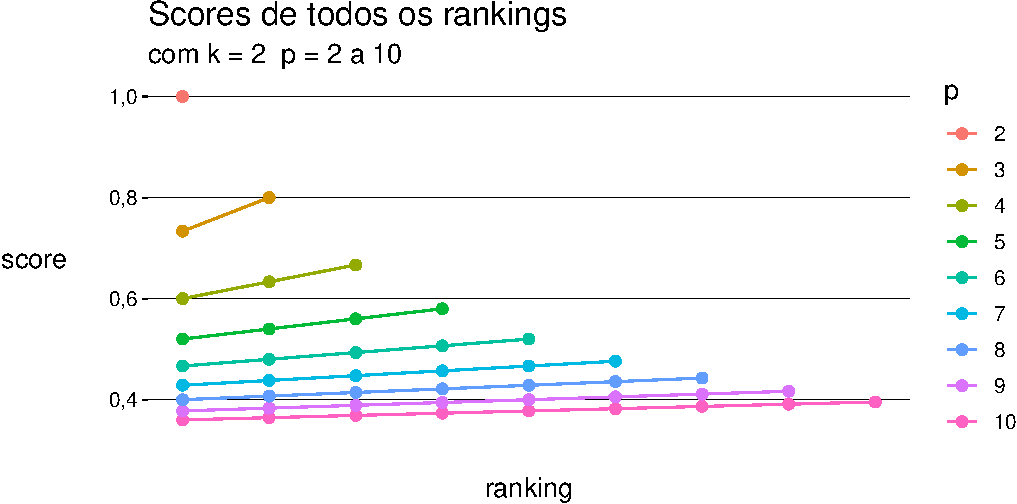
\includegraphics[width=1\textwidth,height=\textheight]{gerar-listas-e-rankings_files/figure-pdf/unnamed-chunk-14-1.pdf}
\end{center}

\begin{Shaded}
\begin{Highlighting}[]
\FunctionTok{criar\_plot}\NormalTok{(r, }\AttributeTok{reta =} \ConstantTok{FALSE}\NormalTok{)}
\end{Highlighting}
\end{Shaded}

\begin{center}
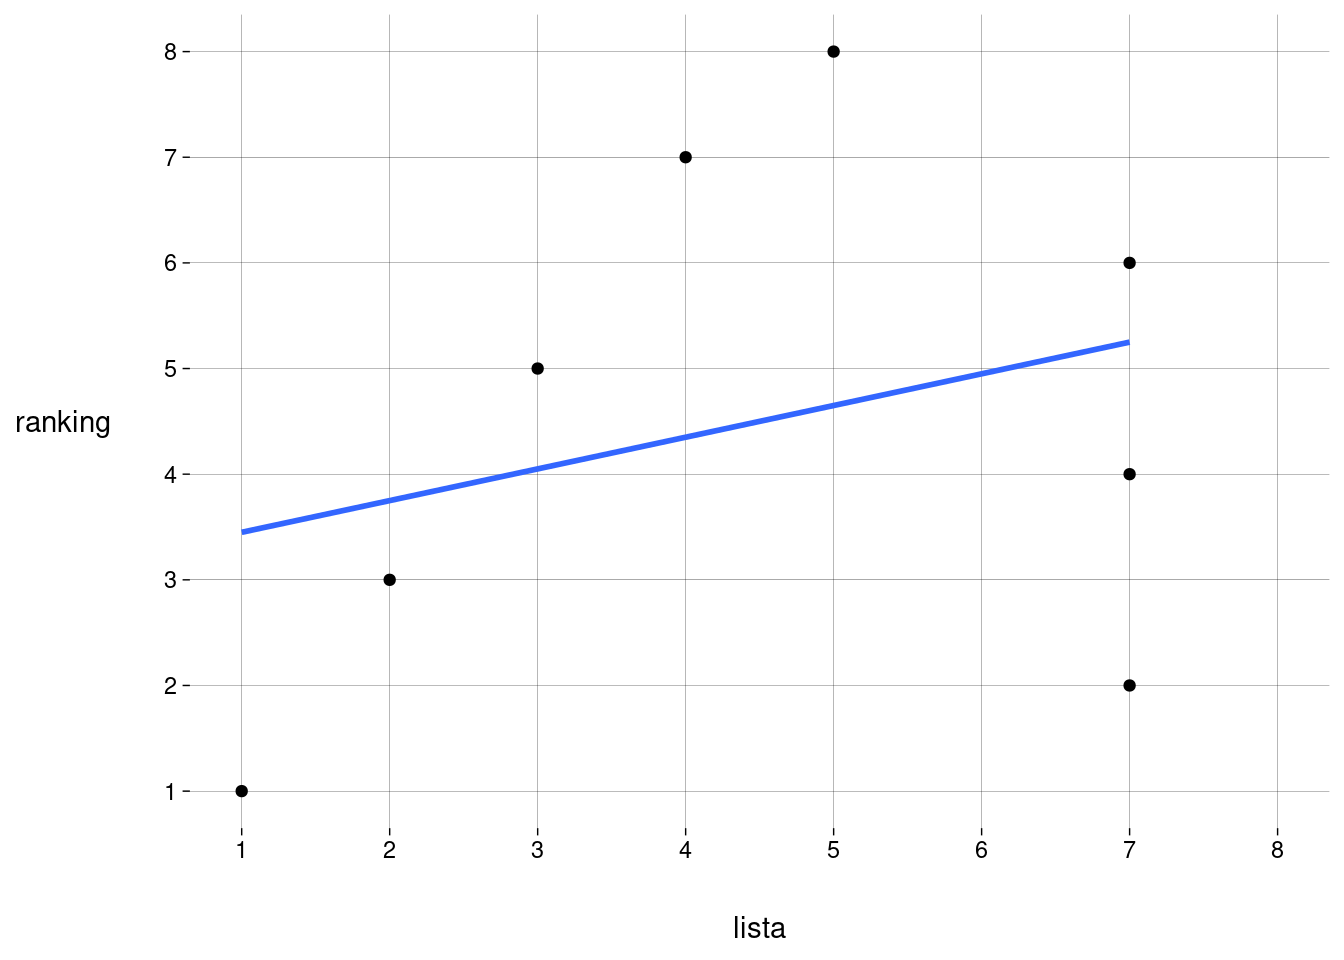
\includegraphics[width=1\textwidth,height=\textheight]{gerar-listas-e-rankings_files/figure-pdf/unnamed-chunk-15-1.pdf}
\end{center}

\begin{Shaded}
\begin{Highlighting}[]
\FunctionTok{criar\_plot}\NormalTok{(r, \textbackslash{}(df) \{ }\FunctionTok{cor}\NormalTok{(df}\SpecialCharTok{$}\NormalTok{pos\_lista, df}\SpecialCharTok{$}\NormalTok{pos\_ranking) }\SpecialCharTok{\%\textgreater{}\%} \FunctionTok{round}\NormalTok{(}\DecValTok{2}\NormalTok{) \})}
\end{Highlighting}
\end{Shaded}

\begin{center}
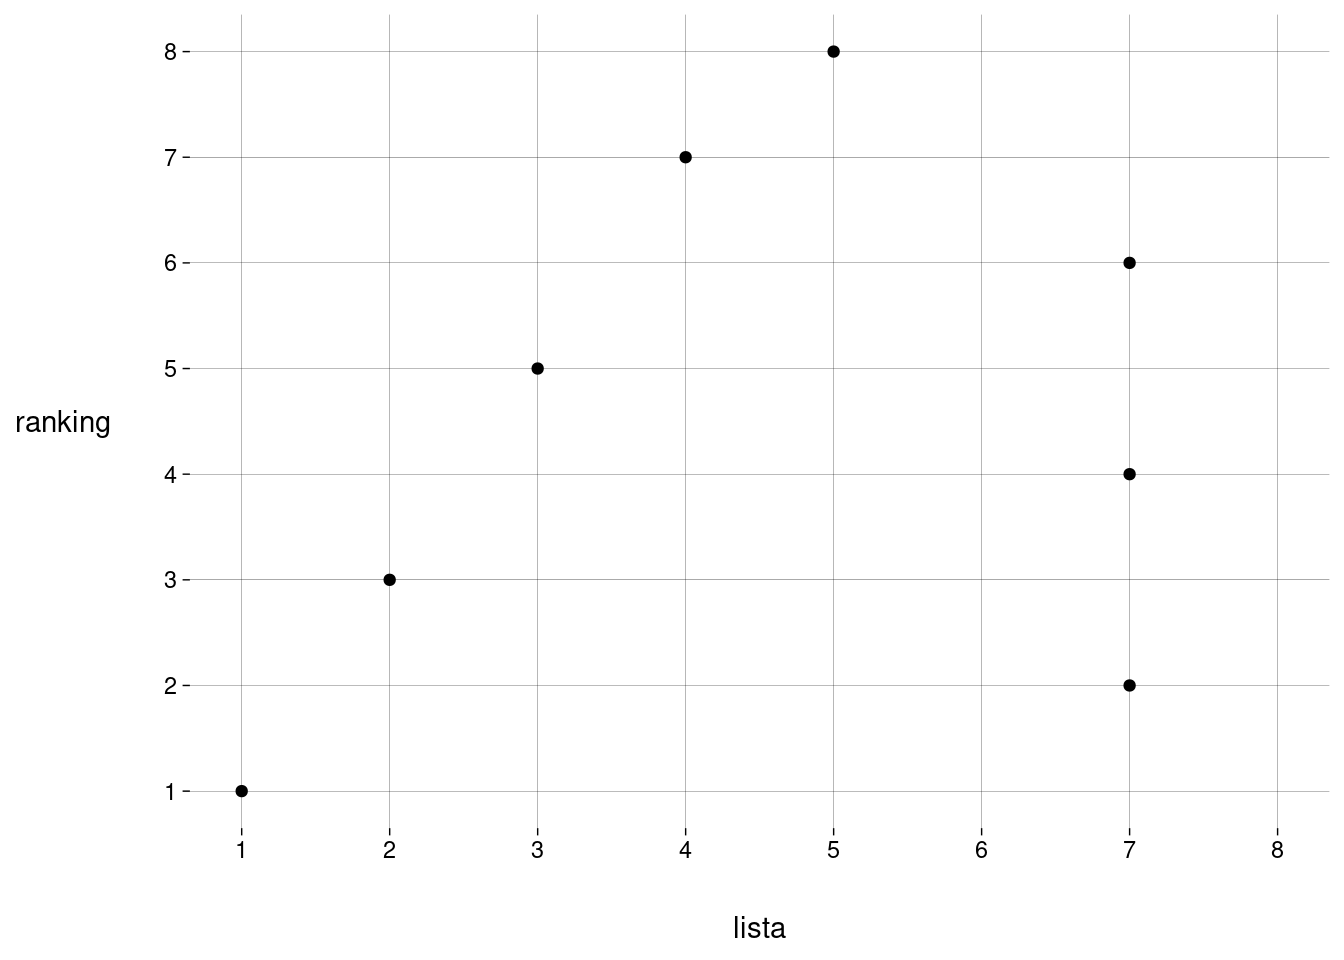
\includegraphics[width=1\textwidth,height=\textheight]{gerar-listas-e-rankings_files/figure-pdf/unnamed-chunk-16-1.pdf}
\end{center}



\end{document}
